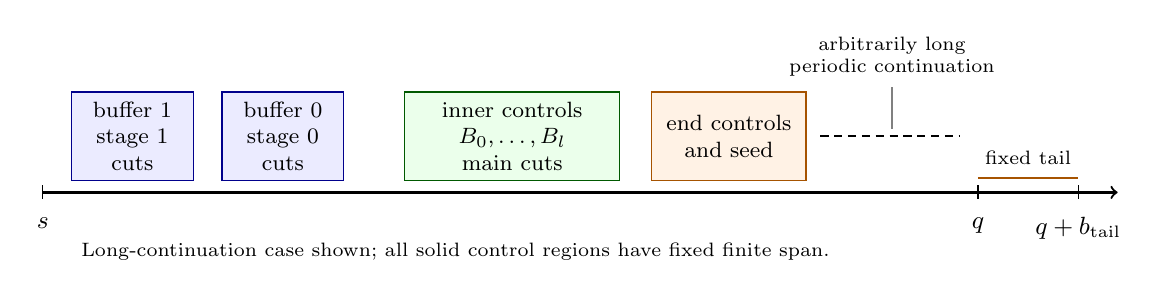
\begin{tikzpicture}[x=0.91cm,y=0.75cm,font=\small]
 \draw[->,thick] (0,0) -- (15,0);
 \draw (0,0.12) -- (0,-0.12) node[below=3pt] {$s$};
 \filldraw[fill=blue!8,draw=blue!55!black]
   (0.4,0.2) rectangle (2.1,1.7);
 \node[align=center,font=\footnotesize] at (1.25,0.95) {buffer $1$\\stage $1$\\cuts};
 \filldraw[fill=blue!8,draw=blue!55!black]
   (2.5,0.2) rectangle (4.2,1.7);
 \node[align=center,font=\footnotesize] at (3.35,0.95) {buffer $0$\\stage $0$\\cuts};
 \filldraw[fill=green!8,draw=green!35!black]
   (5.05,0.2) rectangle (8.05,1.7);
 \node[align=center,font=\footnotesize] at (6.55,0.95)
   {inner controls\\$B_0,\ldots,B_l$\\main cuts};
 \filldraw[fill=orange!10,draw=orange!65!black]
   (8.5,0.2) rectangle (10.65,1.7);
 \node[align=center,font=\footnotesize] at (9.575,0.95) {end controls\\and seed};
 \draw[densely dashed,thick] (10.85,0.95) -- (12.8,0.95);
 \draw[gray] (11.85,1.78) -- (11.85,1.08);
 \node[align=center,font=\scriptsize] at (11.85,2.3)
   {arbitrarily long\\periodic continuation};
 \draw (13.05,0.12) -- (13.05,-0.12)
   node[below=3pt] {$q$};
 \draw[thick,orange!65!black] (13.05,0.25) -- (14.45,0.25);
 \node[font=\scriptsize] at (13.75,0.58) {fixed tail};
 \draw (14.45,0.12) -- (14.45,-0.12)
   node[below=3pt,align=center] {$q+b_{\rm tail}$};
 \node[anchor=west,font=\scriptsize] at (0.4,-1.0)
   {Long-continuation case shown; all solid control regions have fixed finite span.};
\end{tikzpicture}
